\section{Comparison with existing softwares}
In this section we report some results obtained by the comparison between our implementations and other softwares usually installed in common PCs. We want to mention right now that our implementations have no chances to behave as well as any of the professional softwares employed by default by a PC. The reasons are mainly two: the first one is that programs that compress files or folders into archives .ZIP use an advanced algorithm, where the simple LZ77 is enhanced by further coding, in particular by a Huffman code; this combined coding is called LZ77 Deflate, is used by most of the .ZIP compressors and will be shortly described in the following. The second reason is about time: since we execute our program in Matlab, performances are lowered by the infrastructure of the environment and, moreover, \texttt{for} cycles are not very convenient in this particular language. 

\subsection{LZ77 Deflate}
The \textit{deflate} algorithm differs from the simple LZ77 for the final compression of the dictionary through a Huffman code. The description of the basic version of the algorithm can be found in the RFC1951 \cite{deut1}, here we provide only a brief overview of its functioning.
\\

The original file is first split into blocks of data whose maximum length must be $64$ Kbytes. The LZ77 dictionary is generated through the known procedure, with $L_s = 32000$ and $L_c = 258$ bytes. Once the dictionary is generated, it is compressed using a Huffman code; even if we have three types of data to express (\textit{symbol}, \textit{offset} and \textit{length}), we use only two Huffman trees. The first tree is made of $285$ codewords: the first $256$ ($0, \ldots, 255$) stand for literals, that is the symbols (we look at the message as a sequence of bytes), value $256$ indicates the end of the block of data and values $257, \ldots, 285$ are used to indicate the \textit{length} field, which can assume values in $0, \ldots, 258$. Note that some of the \textit{length} codewords are used to represent more than one actual length, for example value $277$ refers to the set of lengths $67, \ldots, 82$. To properly encode a length it is, thus, necessary to attach after the codeword itself a sequence of bits, at most five, which specifies the \textit{length} value among the set described by the codeword. Each value $257, \ldots, 285$ has a fixed number of following bits (from no one to $5$ bits), hence, since Huffman is a prefix code, the receiver can uniquely decode a codeword just by its prefix and then extract the additional information from the following bits without misunderstanding the code. The second Huffman tree is used for the distances between the matched pattern from the beginnning of the \textit{coding window}. Of course, if a \textit{length} is decoded, the receiver knows that the following bits refer to the related \textit{offset}.

Each block of data is preceded by three bits: the first one says whether the current block is the last one; the second and the third specify the type of compression that has been used: not compressed, compressed with fixed and defined Huffman trees or compressed with dynamically generated Huffman trees. If the Huffman code is generated ad hoc, we must also transmit the tree to the receiver to allow a correct interpretation. In general the same set of probabilities can give birth to different Huffman trees, but, specifying some construction rules, we can guarantee the unique correspondence between alphabet and tree. Moreover, a tree generated in such a way can be encoded using only the sequence of the codeword lengths. The Huffman trees are, in turn, compressed combining Huffman and run-length codes. The description of this code is included in the message itself. For a dynamically compressed block of data, the structure of the message is the following:
\begin{itemize}
\item
3 bits to specify whether the block is the last one and how it is compressed;

\item
description of the code used to compress the Huffman tree for \textit{symbols} and \textit{lengths} and the Huffman tree for the \textit{offsets};

\item
compressed Huffman trees for \textit{symbols}, \textit{lengths} and \textit{offsets};

\item
compressed representation of the LZ77 dictionary;

\item
byte $256$ to indicate the end of the block.
\end{itemize}

\subsection{Comparison with \texttt{zip} and \texttt{gzip}}

Combining several steps of compressions it is possible to reach very good performances, also in cases where simple LZ77 or LZSS are not very effective. In the following bar graphs we compare, for each of the seven test files, the compression performances of our implementation of the LZ77 and LZSS algorithms and the Unix versions of the programs \texttt{zip} and \texttt{gzip}:

\begin{center}
\begin{figure}[H]
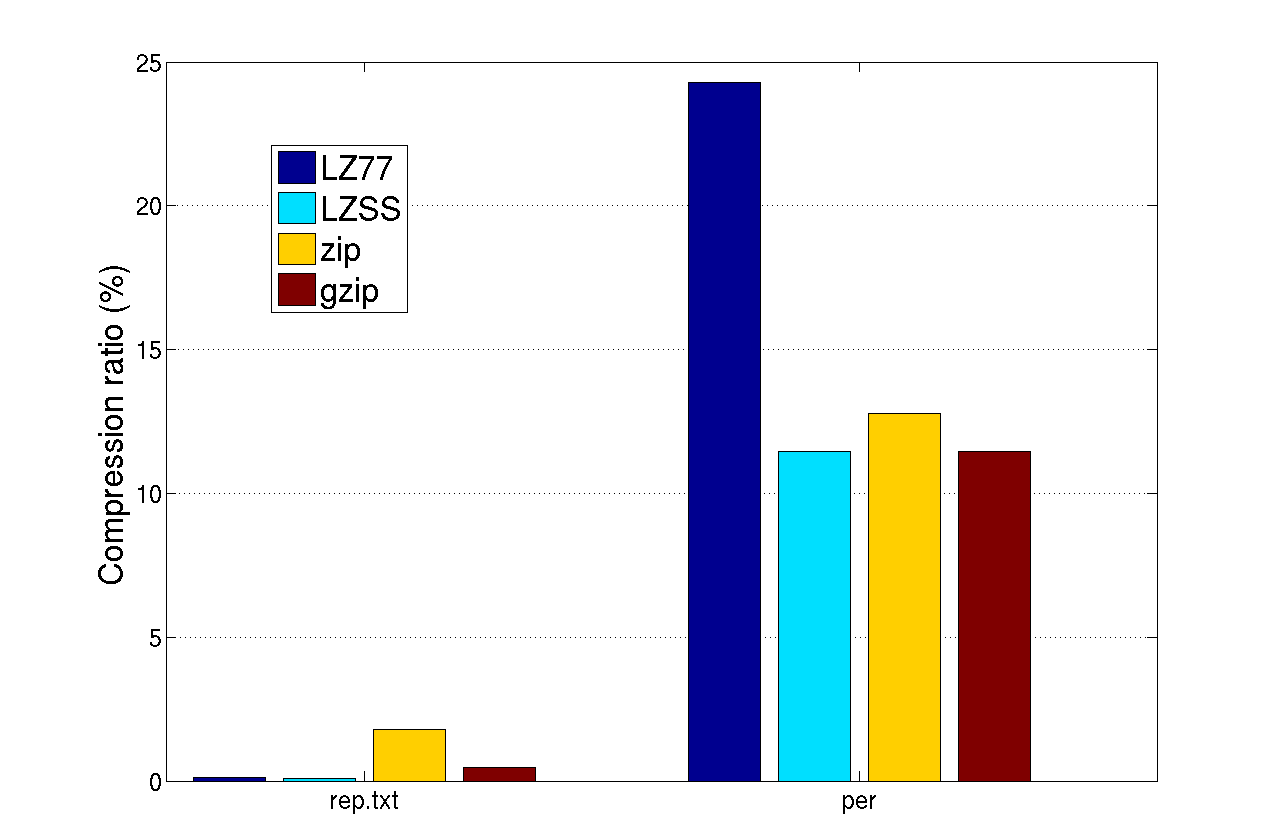
\includegraphics[width=10cm]{images/bars1.png}
\caption{Highly redundant files.}
\end{figure}
\end{center}

\begin{center}
\begin{figure}[H]
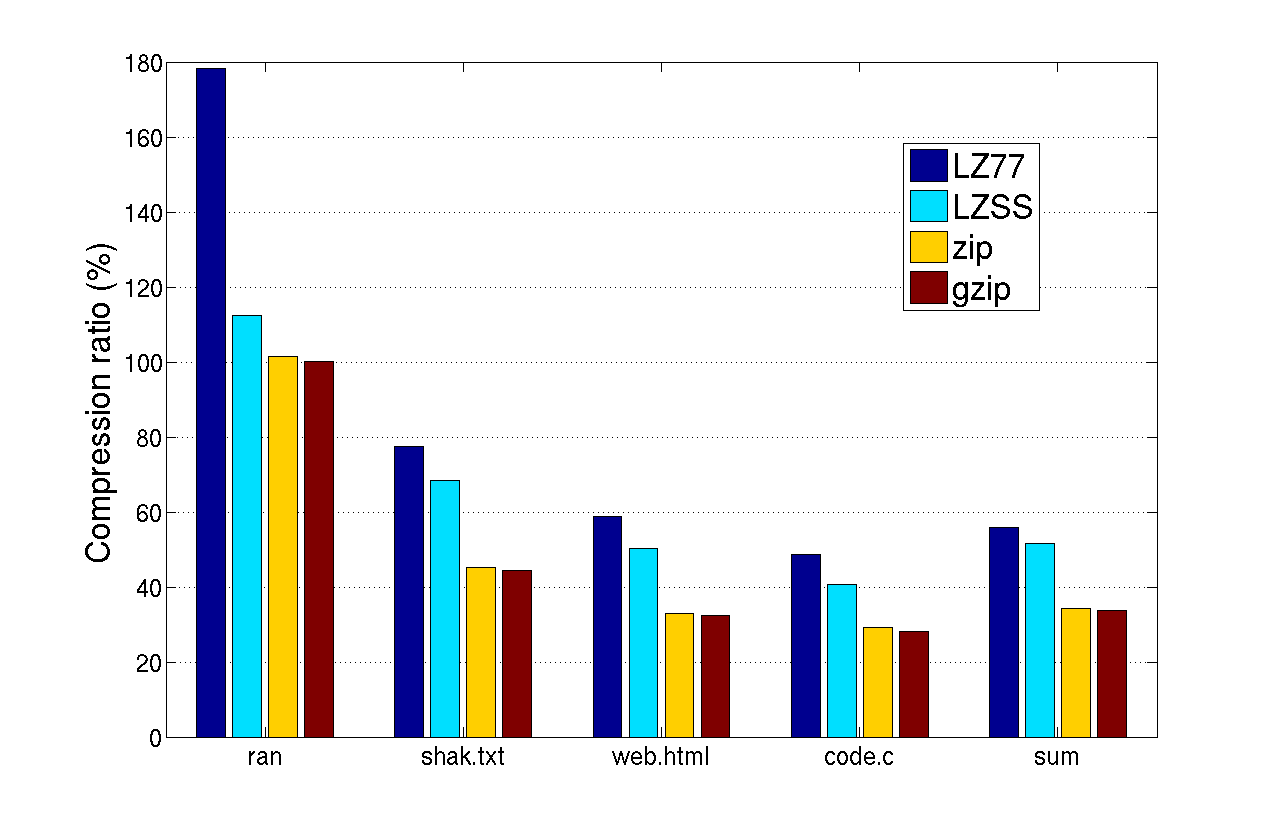
\includegraphics[width=10cm]{images/bars2.png}
\caption{Common files.}
\end{figure}
\end{center}

